\documentclass{article}

\usepackage[a4paper]{geometry}

\usepackage{graphicx}
\graphicspath{{titech/ART.T458.AdvancedMachineLearning/Final2/}}

\usepackage[%
    colorlinks=true,
    pdfborder={0 0 0},
    linkcolor=red
]{hyperref}

\usepackage{latex/common}

\title{Final Report}
\date{2021 August}
\author{Sixue Wang 21M30927\\Tokyo Institute of Technology}

\begin{document}

\maketitle

\section*{Q1}
The sigmoid function is neither convex nor concave, so I would like to use gradient descent to find the optimal value. The loss function of this problem is $||f(x)-g(x)||$. In order to ensure that the optimal $b$ satisfies the constraints in the domain of $f$, I constructed the following dataset:
\begin{CMath}
  X = \{-1.0, -0.9, -0.9, ..., 0.0, 0.1, 0.2, ..., 1.0, 1.1, 1.2, ..., 2.0, 2.1, 2.2, ..., 3.0, 3.1, 3.2, ..., 4.0\} \\
  Y = \{0.0, 0.0, 0.0, ..., 2.0, 2.0, 2.0, ..., -1.0, -1.0, -1.0, ..., 3.0, 3.0, 3.0, ..., 0.0, 0.0, 0.0, ..., 0.0\}
\end{CMath}
I also need to carefully set the initial value of $b$, because $w$ has a huge magnitude and sigmoid is insensitive in that domain which means the wrong initialization will lead gradient vanish or explosion then fail to converge. So I have to give a rough solution and let gradient descent to fine-tune it.
\begin{center}
  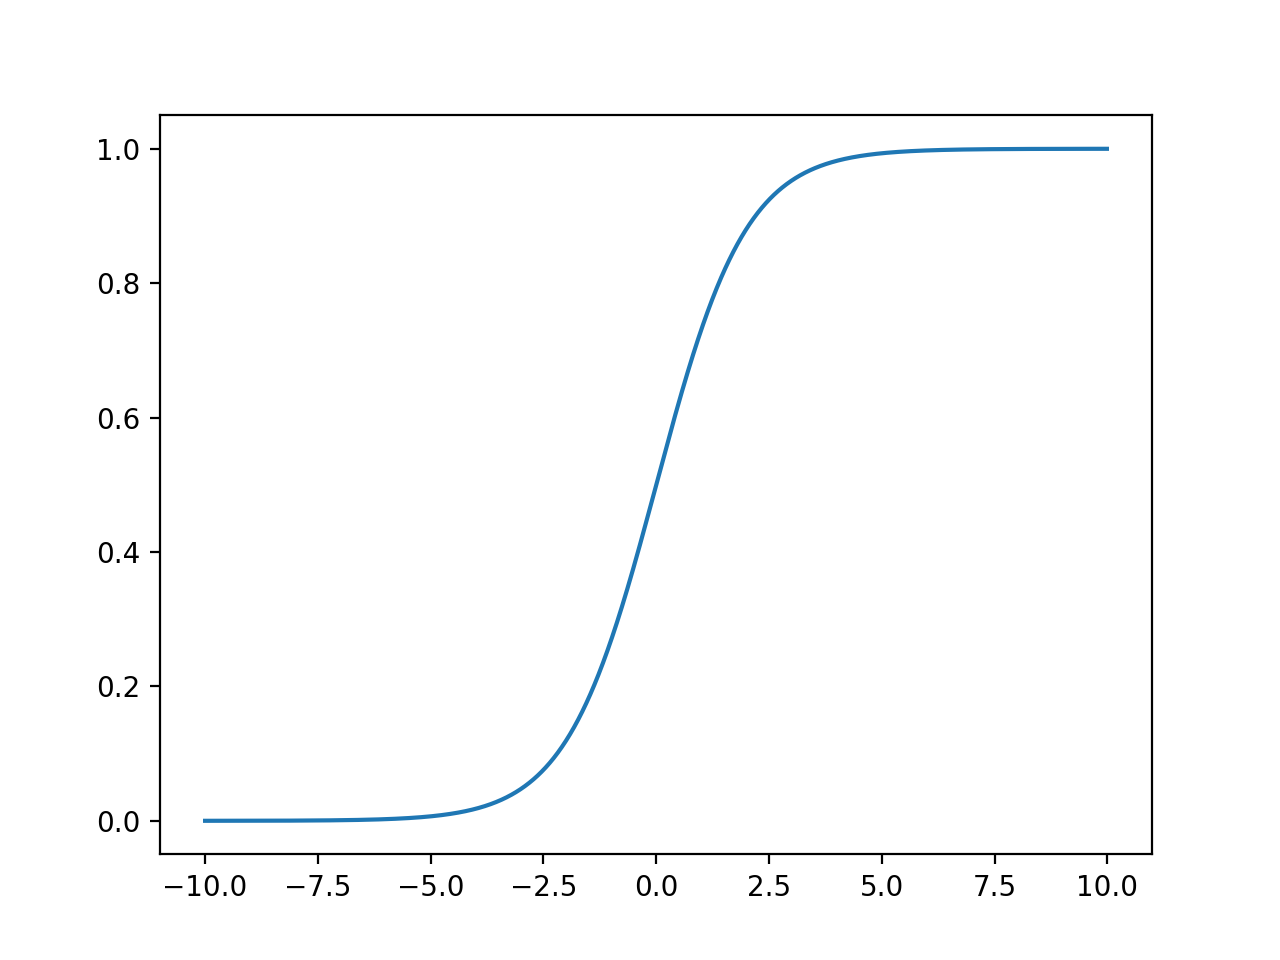
\includegraphics[scale=0.3]{sigmoid}
  \captionof{figure}{sigmoid}
\end{center}
The interesting thing is that $v = [2, -2, -1, 1, 3, -3]$, we can get one possible initialization by solving the following equations:
\begin{CMath}
  \sigma(w_0 * 0 + b_0) \approx 1 \\
  \sigma(w_1 * 1 + b_1) \approx 1 \\
  \sigma(w_2 * 1 + b_2) \approx 1 \\
  \sigma(w_3 * 2 + b_3) \approx 1 \\
  \sigma(w_4 * 2 + b_4) \approx 1 \\
  \sigma(w_5 * 3 + b_5) \approx 1 \\
\end{CMath}
where $b_i$ is decreasing. As $x$ increases, the previous $g_i$ will be offset by the new $g_i$, and the following $g_i$ will always remain 0. In my experiment, I set $b = [5, -995, -995, -1995, -1995, -2995]$ and $\epsilon=1e-4$, the optimal $b=[11.6939,  -988.3085,  -989.0007, -1989.0112, -1987.9169, -2987.8752]$.
\begin{center}
  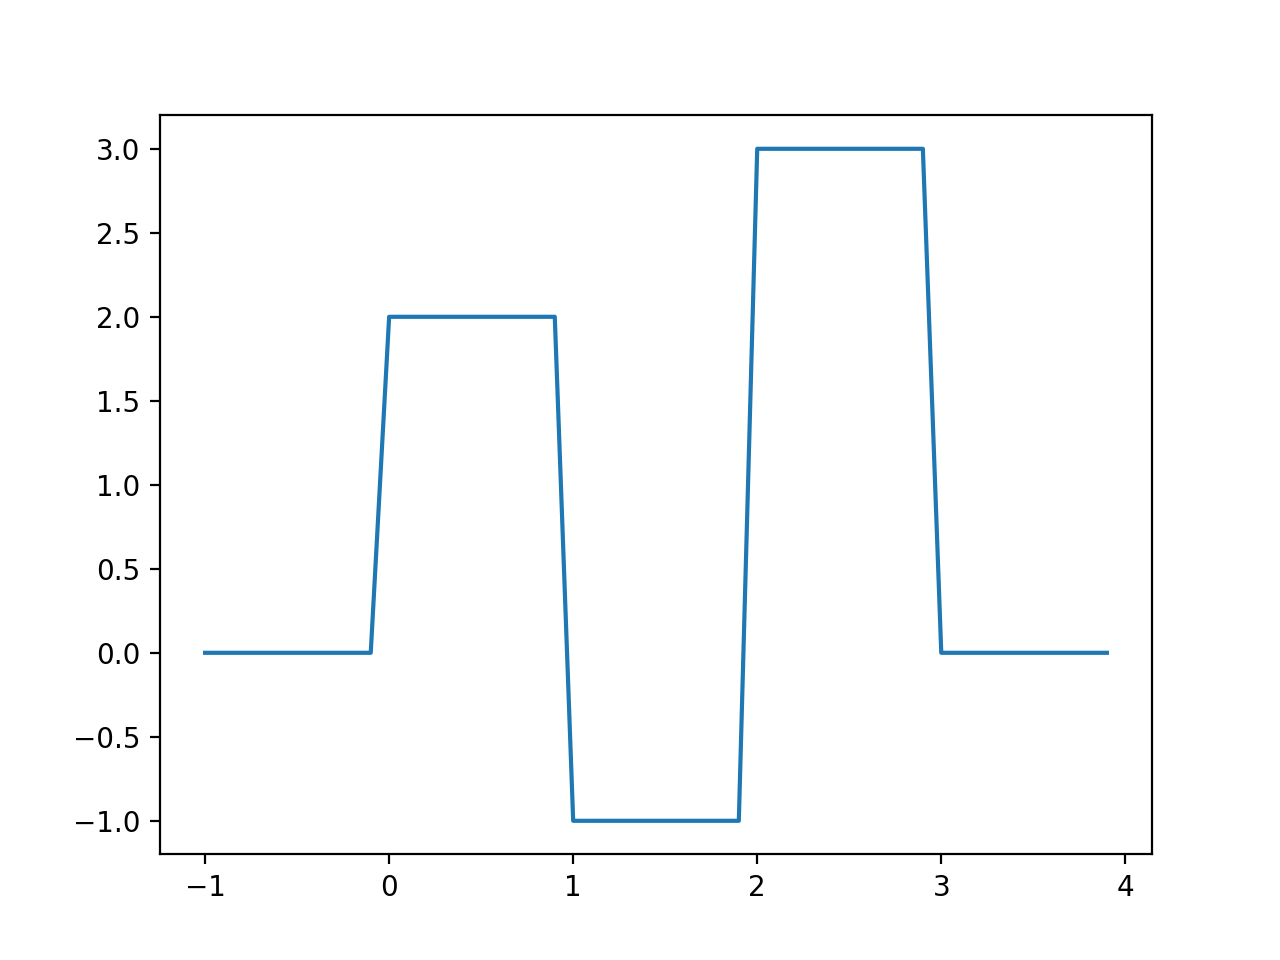
\includegraphics[scale=0.3]{q1}
  \captionof{figure}{g(x)}
\end{center}
\begin{PYCode}[q1 in pytorch]
w = torch.tensor([[1000. for _ in range(6)]])
v = torch.tensor([[2.], [-2.], [-1.], [1.], [3.], [-3.]])
b = [[5., -995., -995., -1995.0, -1995.0, -2995.0]]
b = torch.tensor(b, requires_grad=True)
f = lambda x: torch.sigmoid(x @ w + b) @ v

x = []
y = []
data = [[-1, 0, 0.], [0, 1, 2.], [1, 2, -1.], [2, 3, 3.], [3, 4, 0.]]
for l, r, val in data:
    x += [i for i in np.arange(l, r, 0.1)]
    y += [val for i in range(int((r - l) / 0.1))]
x = torch.tensor(x, dtype=torch.float32).reshape(len(x), 1)
y = torch.tensor(y).reshape(len(y), 1)

for i in range(1000000):
    loss = torch.norm(f(x) - y, p=1)
    loss.backward()
    if loss <= 1e-4:
        break
    with torch.no_grad():
        b -= 10 * b.grad
        b.grad.zero_()
\end{PYCode}

\section*{Q2}
\subsection*{(1)}
\begin{CMath}
  h       & = [0.0, 1.5] \\
  \hat{y} & = [0.5]
\end{CMath}
\subsection*{(2)}
The cross-entropy loss is used to train classification model. In our setting, $y \in R$, so I assume that $\hat{y}$ represents the positive probability, and the negative probability is $1-\hat{y}$. If $y=0$(negative), the cross-entropy loss is
\begin{CMath}
  -(1-\hat{y}) + log(exp(\hat{y})+exp(1-\hat{y})) &= 0.6931 \\
  \frac{\partial loss}{\partial w} &= [[-0.25,-0.25],[0.0,0.0]] \\
  \frac{\partial loss}{\partial b} &= [-0.25, 0.0] \\
  \frac{\partial loss}{\partial q} &= [-0.375, 0.0] \\
  \frac{\partial loss}{\partial c} &= [-0.25] \\
\end{CMath}
\begin{PYCode}[q2 in pytorch]
w = torch.tensor([[1., 1.], [-1., -1.]], requires_grad=True)
b = torch.tensor([-0.5, 1.5], requires_grad=True)
q = torch.tensor([1., 1.], requires_grad=True)
c = torch.tensor([-1.5], requires_grad=True)
h = lambda x: torch.nn.ReLU()(w @ x + b)
y = lambda x: torch.nn.Sigmoid()(h(x).T @ q + c)

x = torch.tensor([0., 0.])
print("h = {}".format(h(x)))
print("y = {}".format(y(x)))

x = torch.tensor([1., 1.])
loss = -(1. - y(x)) + torch.log(torch.exp(y(x)) + torch.exp(1.0 - y(x)))
loss.backward()
print("loss = {}".format(loss))
print("gw = {}".format(w.grad))
print("gb = {}".format(b.grad))
print("gq = {}".format(q.grad))
print("gc = {}".format(c.grad))
\end{PYCode}

\section*{Q3}
\begin{itemize}
  \item \href{https://arxiv.org/pdf/1608.00869.pdf}{SimVerb-3500} defines a word similarity task. It contains 3500 verb pairs whose similarity is rated by human. If we don’t pay attention to the philosophy behind this dataset, we can evaluate the quality of word embeddings directly by calculating the similarity(cosine function) for all questions and the average can be thought of the accuracy.
  \item \href{https://arxiv.org/pdf/1301.3781.pdf}{Google Dataset} defines a word analogy task. The section 4.1 in this paper gives a detailed description. There 8869 semantic and 10675 syntactic questions in this dataset. Each question consists of a pair of similar words.  Word analogy represents the relations between of words and the good representation could satisfy numerical calculations, for example, $Paris - France + Italy = Rome$. Now we can define the loss by $Diff(Paris - France + Italy - Rome)$ where $Diff$ can be any distance formula, such as Euclidean distance..
\end{itemize}

\section*{Q4}
\begin{itemize}
  \item Transformer can naturally support parallel computing. What I mean is that any element in the sequence only depends on the features of the previous layer and does not rely on other elements in the same layer. If we only look at Transformer's underlying implementation, we will find that every operation is a matrix multiplication, so we can easily stack hardware to improve efficiency. But RNN, in order to extract timing/sequence information, has to collect the previous elements' feature to caculate the current one. This means that the critical path of computation cannot be accelerated in parallel. However, increasing the batch size can still improve the throughput of processing.
  \item Also due to the structure of RNN, the problem of gradient vanish often occurs during training. Although tanh can lessen to a certain extent, it is still not so easy to make RNN converge, especially when the sequence length is too long. The Transformer captures sequence information through self-attention. In theory, as long as the hardware resources can be satisfied, it can handle infinitely long sequences.
\end{itemize}

\section*{Q5}
The hypothesis of this paper is that meta-learning can overcome the shortcoming of fine-tune method. It tries to learning lots of different abilities during pre-training time, and then adapts to downstream tasks by indicating what the task it is. Its advantage is that when inferencing downstream tasks, only little or no examples are showed without gradient update. It can break through the limitation of the fine-tune method relying on large amounts of data. At the same time, this way of learning is more similar to that of humans.

To confirm this hypothesis, they trained GPT-3 which has 175 billion parameter and see the meta-learning performance on two dozen NLP datasets. The GPT-3 is evaluated over all datasets under 3 conditions:
\begin{itemize}
   \item few-shot: the task description and about 10-100 examples will be demonstrated to GPT-3;
   \item one-shot: the task description and only one examples will be demonstrated to GPT-3;
   \item zero-shot: only the task description will be demonstrated to GPT-3;
\end{itemize}
Generally speaking, GPT-3 can achieve compatible or surpassed performance with state-of-the-art method on all tasks. Although one-shot and zero-shot are not as good as few-shot, they still show potential possibilities.

GPT-3 is a Transformer-based model which only stackes decoder block. The original text will pass tokenization first, then goes through the word embedding layer. The final input is the sum of word embedding and position embedding. This input will be processed by several Transformer-decoder which has only masked sparse self-attention layers and alternating feed forward layers. "masked" means the attention mechanism will only operate on the embedding before the curren time and "sparse" means factoring the attention matrices to reduce the computational cost. The output of the decoder will product with the word embedding matrix again to get the probability of words. As for the dimension of embedding, the number of decoders, the number of neurons in the hidden layer, and the number of attention heads can all be specified arbitrarily. In their paper, they trained 8 different sizes of GPT-3 from 125M parameters to 175B parameters.

The training dataset sources from Common Crawl dataset2 which has nearly a trillion words. In order to improve the quality of this dataset further, they also introduce 3 more steps:
\begin{itemize}
   \item filtering based on similarity to a range of high-quality reference corpora;
   \item fuzzy deduplication at the document level, within and across datasets;
   \item adding known high-quality reference corpora.
\end{itemize}

In general, this paper carried out 9 categories of experiments: Language modeling, QA, Translation, Winograd-Style Tasks, Common Sense Reasoning, Reading Comprehension, SuperGLUE, NLI, and Synthetic and Qualitative Tasks. GPT-3 has achieved the best results on some tasks, but in some other dataset, GPT-3 is significantly worse than other SOTA methods, such as Common Sense Reasoning. The author believes that this may be caused by data contamination. On the other hand, few-shot are always better than the other two and increasing model parameters can also improve accuracy.

Although GPT-3 has achieved good results, there are also some unsatisfactory places:
\begin{itemize}
  \item On text synthesis, GPT-3 maybe generates redundant and meaningless content;
  \item The structure of GPT-3 is unidirectional which leads bad performance in fill-in-the-blank tasks;
  \item The objective weights every token equally and lacks a notion of what is most important;
  \item Poor sample efficiency during pre-training;
  \item It is impossible to explain whether the excellent results of few-shot are due to pre-training or the provided examples;
  \item heavy inference time.
\end{itemize}
\end{document}
